\chapter{RQA systém firmy Y Soft}
\label{rqa}

Robotic Quality Assurance (dále jen RQA) je systém postavený na robotice a počítačovém vidění sloužící k~automatizaci testování zařízení nejen s~dotykovým displejem, ale i hardwarovými prvky. Jeho aktuálně primárním účelem je testování tiskáren a hlavního produktu firmy Y~Soft, kterým je Y~Soft SafeQ. Řešení by nicméně šlo použít na většinu dotykových a vestavěných aplikací.

\section{Význam RQA pro firmu Y Soft}
Hlavním důvodem vzniku RQA bylo usnadnění práce vývojářům a QA inženýrům s~vykonáváním opakovaných, časově náročných a manuálních operací. Ať už se programuje software do tiskáren, jako je tomu v~případě Y~Softu, nebo de facto do čehokoliv jiného, musí pak přijít tester, který aplikaci podle zadaného scénáře ručně otestuje. Tento postup se typicky opakuje při každém vydání nové verze. U~čistě softwarových systémů a aplikací lze tento proces alespoň zčásti automatizovat pomocí RPA, avšak samostatným zařízením, kterými jsou právě například tiskárny, se manuální proces testování nevyhne.

Úkolem RQA je manuální testování odstranit. Proč by měl stále stejné a~opakující se akce dělat člověk a~ne robot? S~dnešními technologiemi umělé inteligence a počítačového vidění toho lze dosáhnout. V~principu se samotný proces testování v ničem nemění. Místo člověka pouze stojí před zařízením kamera s~robotický ramenem jako na~obrázku~\ref{robot-img}, které je schopno klikat na displej a tlačítka stejně dobře jako člověk.

\begin{figure}[hbt]
	\centering
	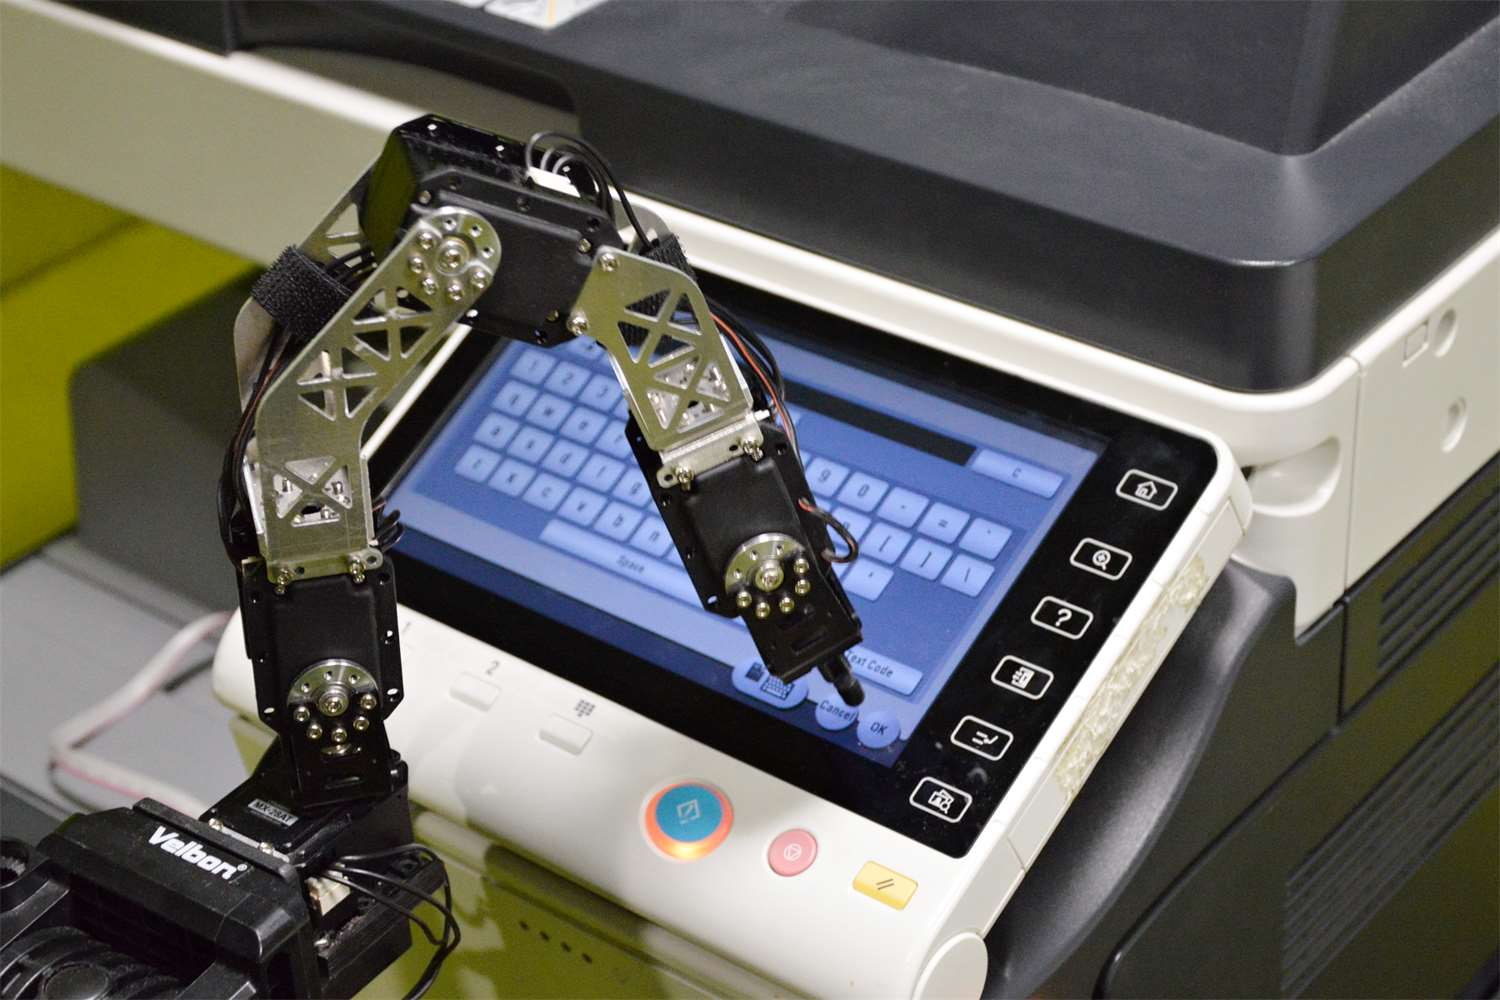
\includegraphics[width=1\textwidth]{obrazky/robot.png}
	\caption{Robot systému RQA v~průběhu testování tiskárny}
	\label{robot-img}
\end{figure}

Automatizace testování přináší mnoho výhod. Jednou z nich je ušetření nákladů, neboť testuje-li robot, není třeba platit člověka. Dále značně usnadňuje práci softwarovým vývojářům, kteří tímto způsobem šetří čas a mohou se věnovat důležitějším věcem. Roboty lze navíc nechat testovat přes noc a během dne se již jen zabývat výsledky a řešením problémů. Toto opět šetří čas a zrychluje celý proces testování. Za~následek to má rychlejší zpětnou vazbu vývojářům testovaného produktu, tedy i opravu chyb, a ve~výsledku dřívější vydání nové verze.

Mimo jiné roboti umožňují vzdálené ovládání cílového zařízení. Tato vlastnost otevírá dveře mnoha novým využitím. Vývojářům, kteří se jinak nemohou hnout od tiskáren, dává možnost pracovat z~domova či prakticky odkudkoliv. Zařízení a roboty lze spravovat lokálně a zákazníci pak mohou se~systémem pracovat na dálku odkudkoliv na světě. Stejným způsobem lze nabízet služby potenciálním zákazníkům na zkušební dobu, u~kterých instalace robota na pár týdnů nedává smysl. Vzdálené sdílení robotů navíc redukuje cenu vybavení až o~30~\% a snižuje čas potřebný pro připravení systému k~použití.

Skutečnou představu o~významu RQA pro Y~Soft lze však získat až z~čísel:
\begin{itemize}
  \item přes 1000 automatických testů,
  \item až 5x rychlejší proces testování,
  \item pokrytí testy zvýšeno o~200~\%,
  \item snížení nákladů na QA o~více než 30~\%,
  \item 98~\% vývojářů může pracovat vzdáleně,
  \item pětinásobně vyšší ROI v~porovnání s~manuálním testováním.
\end{itemize}

Nezanedbatelným přínosem RQA je i reklama firmě, neboť roboti jsou poměrně atraktivní a již existuje nejeden článek o~liduprázdných kancelářích jen s~pracujícími roboty.

\section{Architektura}
Systém je implementovaný na platformě .NET v~jazyce C\# a sestává z~několika částí. Jak je znázorněno na obrázku~\ref{rqa-architecture-img}, u~testovaného zařízení musí stát kamera, která snímá obraz a posílá ho dál ke~zpracování. Služby na backendu tento zpracovávají a komunikují s~robotem, který pak vykonává dané akce. Uživatel se~systémem interaguje pomocí webového rozhraní a samotné testy vytváří v~test frameworku. Záznamy o~událostech v~RQA jsou ukládány v~centrálním logovacím systému Graylog.

\begin{figure}[hbt]
	\centering
	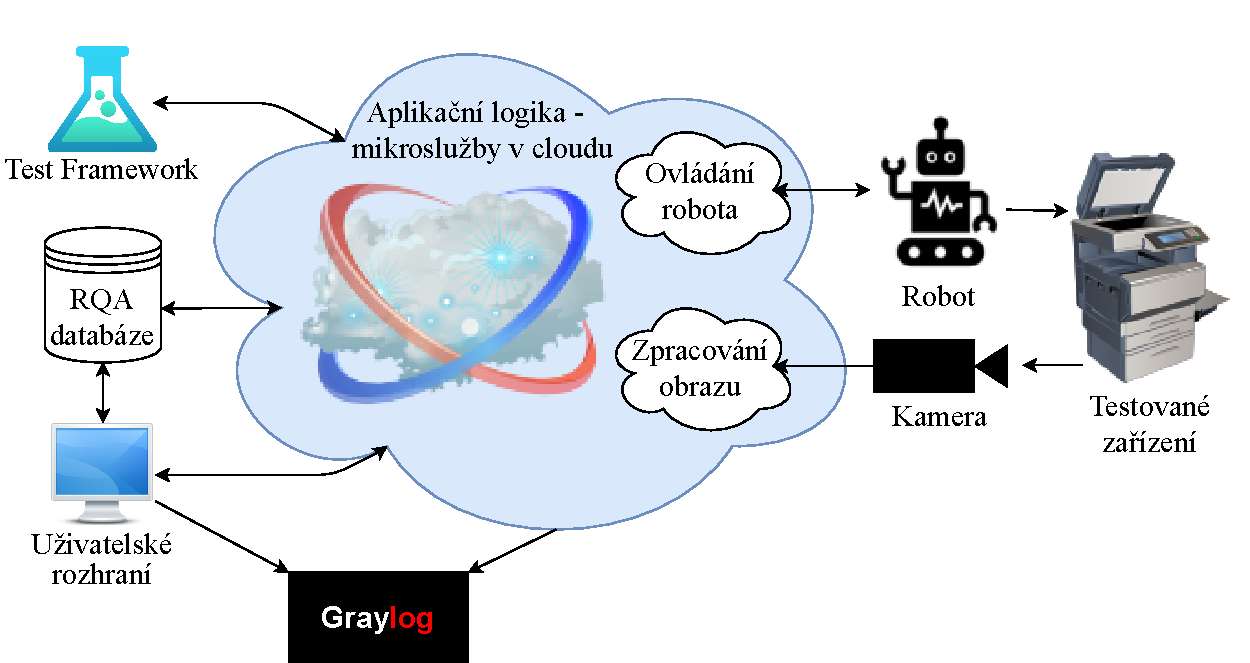
\includegraphics[width=1\textwidth]{obrazky/rqa-architecture.pdf}
	\caption{Vysokoúrovňová architektura RQA systému}
	\label{rqa-architecture-img}
\end{figure}

Pro~tuto práci jsou relevantní zejména mikroslužby aplikační logiky a systém Graylog. Vzhledem k~architektuře mikroslužeb má každou doménu (zpracování dat, počítačové vidění apod.) či subdoménu na starost zcela samostatná služba. Služby spolu komunikují prostřednictvím zpráv skrze RabitMQ. Právě tato architektura je jedním z~hlavních důvodů pro~potřebu detekce anomálií, neboť některá služba může mít problém, který ji třeba zpomaluje, aniž by si toho někdo všiml. U~monolitického systému by se tato skutečnost projevila mnohem výrazněji, neboť by ovlivnila systém jako celek. Systému Graylog je pak věnována zvláštní kapitola~\ref{graylog}.